% ----------------------------------------------------------
\chapter{Proposed Method}
% ----------------------------------------------------------

\section{Fret requirements}
% Still need to explain what is fret

In prior effort to elaborate safety monitoring requrements for the ProVANT project, 
team members
% , specially from UFSC and % What other university?
have proposed around 66 Fret requirements, for each of the control boards and for the systema as a whole. These requirements can be grouped in five topics:
\begin{enumerate}
	\item Execution time (some specific to the control loop, like \textcolor{orange}{upon ControlLoopStart} \textcolor{green}{System shall} \textcolor{cyan}{within 6 milliseconds} \textcolor{blue}{satisfy ControlAlgorithmFinish}, others to every thread)
	\label{item:exec_time}
	
	\item Monitoring and transmission of data necessary to the control algorithm.
	\label{item:mon_trans}

	\item The transition between controllers
	
	\item If the monitors are active (like in \textcolor{red}{while SimulationMode | RealMode} \textcolor{green}{Nucleo shall} \textcolor{cyan}{always} satisfy \textcolor{blue}{ServoMonitoring \& BatteryMonitoring \& AttitudeMonitoring})
	
	\item Fault detection
\end{enumerate}

A possible solution to the \autoref{item:exec_time} item is proposed by \textcite{broering_runtime_2023}, with the library that he developed called \gls{RMLib}. This library helps to record time stamps of begining and ending of periods of interest (proposed to be used to monitor threads execution time) and compare them with the expected \gls{WCET} and a deadline. It allows for both online and offline monitoring, where in the offline mode it just records the timestamps and streams it to a computer to be recorded and analysed afterwards. 
If used for the porpose of monitoring the control algorithm execution time (as the specification of \autoref{item:exec_time}), the online mode can be used in order to provide the verdicts to a unified monitor software, like the R2U2, but it would increase the over head in the system. \autoref{fig:rmlib_on_off} presents a comparrison between both operation modes.

\begin{figure}
	\caption{\label{fig:rmlib_on_off} Online and offline modes in \gls{RMLib} diagram}

	\begin{center}
		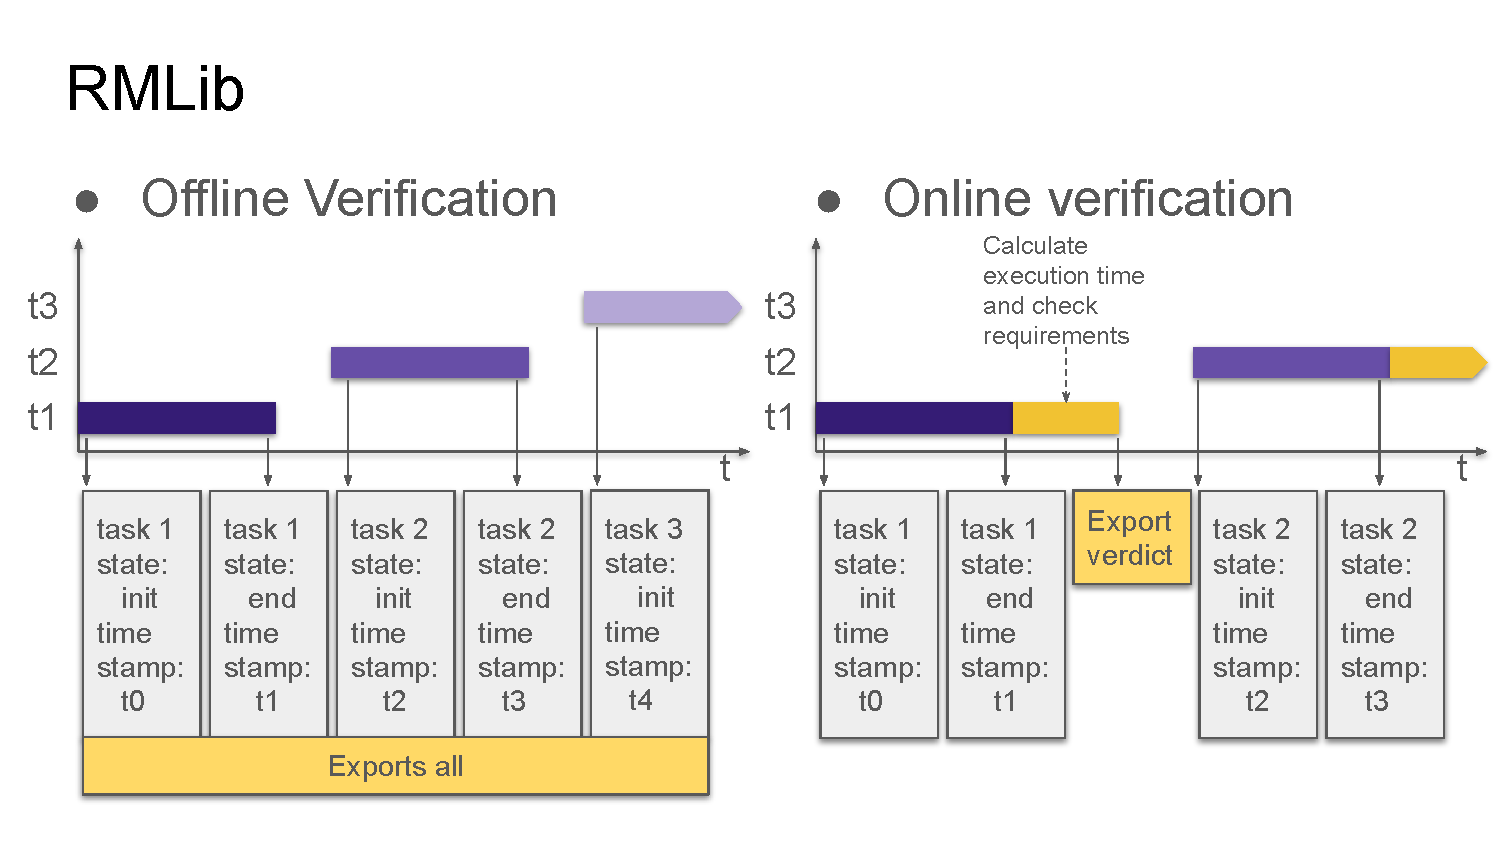
\includegraphics[width=\linewidth,trim=0cm 0cm 0cm 3cm,clip]{images/RMLib_online-offline_comparrison.pdf}
	\end{center}
	% \legend{Source: Own elaboration}
	\fonte{Own elaboration}
\end{figure}

The correct operation of \gls{RMLib} could be used to monitor the requirement 
% \textcolor{orange}{when ControlLoopFinish} \textcolor{green}{System shall} \textcolor{blue}{satisfy CollectHardwareExecutionTimes & AssessHardwareTimePerformance}
\textcolor{orange}{when ControlLoopFinish} \textcolor{green}{System shall} \textcolor{blue}{satisfy CollectExecutionTimes \& AssessTimePerformance} or it could split the requirement in more specific ones for each monitored thread. If offline mode is preferred, it would be more precise to define the requirement as "collect time stamps" or simply "monitor execution time" for monitoring it \gls{RMLib} is running.

The \autoref{item:mon_trans} groups requirements that asks for both transmitting the aquired data and monitoring it, for example \textcolor{red}{while MonitoringEnabled} \textcolor{green}{Nucleo shall} \textcolor{cyan}{always} \textcolor{blue}{satisfy MonitorTiltAngles}. It begs the question if it should be the same requirement, or two separete. Maybe it's desired that the Nucleo should tests the validaty of the data before sending to Jetson, or forwarding to the control thread, in case the Nucleo is in control. It would add a delay to the information flow for the control loop and also, if the read data is not validated, some procedure should be define. How would the controller calculate the next control signal with a missing data? It could simply use the received data from the last time stamp, considering that it should be only slightly diferent than the atual velue.

During the software development some projectist proposed to not use mutexes nor semaphores in the low level software due to it's performances implications, under the premise that the control algorithm should be robust enough to withstand possible faulty data from time to time. Over this such assumptions, it would be an option to just send the data read from the sensors, even if it failes the tests, or not testing them at all before transmission. This decision is however questionable, as there is no guarantee that the data won't be corrupted consecutive times or with a high frequency that would be harmfull to the controller.% \cite{noauthor_software_2024} % isso é bem estranho, não sei se eu gosto desse parágrafo

Moreover, there was no requirements defined to assess the validity of the sensors readings. Redundant sensors or the response of the sensor to the \gls{UAV} motion can be used as a method to verify the validity of the read data, like done in \textcite{bonakdarpour_runtime_2014}.

% \textbf{Instruções da Coordenação do PFC:}

% Neste capítulo, deve-se apresentar:
% \begin{itemize}
% 	\item A solução proposta para o problema descrito no capítulo anterior;
% 	\item Explicar a metodologia utilizada na solução proposta;
% 	\item Deixar bem claro e justificar tecnicamente para o leitor como que a solução proposta resolve o problema abordado e atende aos requisitos técnicos, explicando tecnicamente as decisões que foram tomadas para se chegar a tal solução.
% \end{itemize}

% Sugere-se colocar uma diagrama/fluxograma/casos de uso/etc ilustrando a solução proposta, e depois explicar em detalhes cada parte/bloco do diagrama/fluxograma ao longo do texto. 

% Ressaltamos que, em princípio, há uma infinidade de soluções possíveis para o problema abordado no PFC. Desse modo, é preciso explicar detalhadamente e justificar tecnicamente a solução proposta no PFC.